\documentclass{article}

\usepackage[english]{babel}
\usepackage[a4paper,top=2cm,bottom=2cm,left=3cm,right=3cm,marginparwidth=1.75cm]{geometry}

\usepackage{amsthm}
\usepackage{amsmath}
\usepackage{graphicx}
\usepackage{xcolor}
\usepackage{svg}
\usepackage[normalem]{ulem}

\usepackage{csquotes} % recommended to fix warning
\usepackage[style=alphabetic,sorting=ndt]{biblatex}
\addbibresource{sources.bib}

\usepackage{float}
% \usepackage{subcaption}

\usepackage{tikz}
\usetikzlibrary{matrix, positioning}

\title{Pentomino Pathfinding}
\author{Steven Nguyen (icecream17)}

% pentomino colors
\definecolor{colorI}{HTML}{EEAAAA}
\definecolor{colorF}{HTML}{DDBB99}
\definecolor{colorL}{HTML}{CCCC88}
\definecolor{colorP}{HTML}{BBDD99}
\definecolor{colorN}{HTML}{AAEEAA}
\definecolor{colorT}{HTML}{99DDBB}
\definecolor{colorU}{HTML}{88CCCC}
\definecolor{colorV}{HTML}{99BBDD}
\definecolor{colorW}{HTML}{AAAAEE}
\definecolor{colorX}{HTML}{BB99DD}
\definecolor{colorY}{HTML}{CC88CC}
\definecolor{colorZ}{HTML}{DD99BB}

% tetromino colors
% = colorU
\definecolor{color4I}{HTML}{88CCCC}

% \theoremstyle{plain} % default
\theoremstyle{definition} % not semantic, but removes italics
\newtheorem{theorem}{Theorem}[section]
\newtheorem{corollary}{Corollary}[theorem]
\newtheorem{lemma}[theorem]{Lemma}

\newtheorem{definition}[theorem]{Definition}
\newtheorem{property}[theorem]{Property}

% \theoremstyle{remark} % not semantic to not have this, but keeps bold
\newtheorem*{conclusion}{Conclusion}
\newtheorem*{note}{Note}

\newcommand{\minordetail}[1]{\textcolor{gray}{#1}}
\newcommand{\newterm}[1]{\textit{#1}}
\newcommand{\badterm}[1]{\textcolor{red}{\uwave{\textcolor{black}{#1}}}}

% place at end
\usepackage[colorlinks=true, allcolors=blue]{hyperref}

\begin{document}
\maketitle

% \begin{abstract}
% Your abstract.
% \end{abstract}

\tableofcontents





\section{Introduction}

\cite{v1} posed the following problem: Given a rectangular $n \times m$ grid of squares, place a subset of the twelve pentominoes (see Figure \ref{fig:pentominoes}), and endpoints A and B on the grid \minordetail{without overlaps} such that $\#^{p}_{n, m}$ = the length of (the shortest \minordetail{nonempty, orthogonal} path between $A$ and $B$) is maximized.

The above notation is for the maximum length of any path given some placements $p$; the maximum length given all possible placements is denoted by $\#_{n, m}$, and when $n = m$, the notation is $\#_n$.

\begin{figure}[!h]
    \centering
    \includesvg[width=0.5\linewidth]{All_18_Pentominoes.svg}
    \caption{The twelve pentominoes and their reflections \cite{pentominoes};
    from left-to-right they are named I, F, L, P, N, T, U, V, W, X, Y, Z,
    where F, L, P, N, Y, Z are chiral and have their reflections shown.}
    \label{fig:pentominoes}
\end{figure}






\section{Small grids}

\subsection{No pentominoes}

For $n$ = 1 and 2, $n \times n < 5$, so no pentomino can fit: $\#_1 = 1, \#_2 = 3$.
For $n$ = 3, 9 squares minus a pentomino is 4 squares, so the length 5 path is optimal: $\#_3 = 5$.% (Figure \ref{fig:no123})

\begin{figure}[!h]
    \centering
    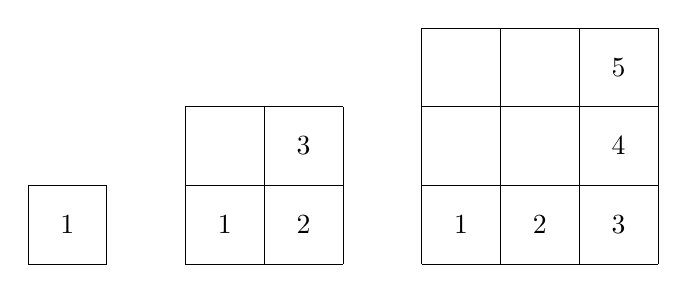
\begin{tikzpicture}
        \draw[step=1cm,black,very thin] (0,0) grid (1,1);
        \draw (0.5,0.5) node{1};

        \draw[step=1cm,black,very thin] (2,0) grid (4,2);
        \draw (2.5,0.5) node{1};
        \draw (3.5,0.5) node{2};
        \draw (3.5,1.5) node{3};

        \draw[step=1cm,black,very thin] (5,0) grid (8,3);
        \draw (5.5,0.5) node{1};
        \draw (6.5,0.5) node{2};
        \draw (7.5,0.5) node{3};
        \draw (7.5,1.5) node{4};
        \draw (7.5,2.5) node{5};
    \end{tikzpicture}
    \label{fig:no123}
\end{figure}

Similar reasoning holds for $n = 2$, $m \le 6$: there is a path of length $m + 1 \le 7$, while $2m - 5 \le m + 1 \le 7$, so you cannot do any better than placing nothing. It turns out there is enough room for the I piece, and so there are two solutions ignoring symmetry:

\begin{figure}[!h]
    \centering
    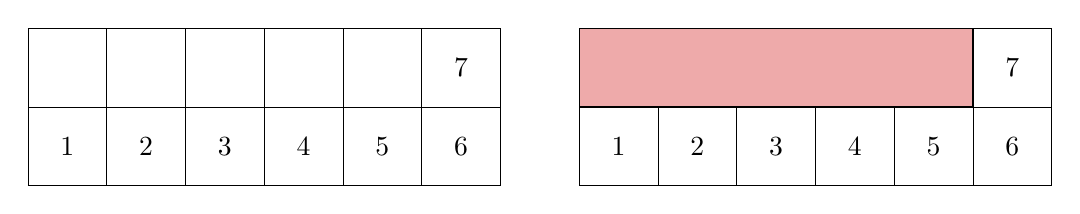
\begin{tikzpicture}
        \draw[step=1cm,black,very thin] (0,0) grid (6,2);
        \draw (0.5,0.5) node{1};
        \draw (1.5,0.5) node{2};
        \draw (2.5,0.5) node{3};
        \draw (3.5,0.5) node{4};
        \draw (4.5,0.5) node{5};
        \draw (5.5,0.5) node{6};
        \draw (5.5,1.5) node{7};

        \draw[step=1cm,black,very thin] (7,0) grid (13,2);
        \draw (7.5,0.5) node{1};
        \draw (8.5,0.5) node{2};
        \draw (9.5,0.5) node{3};
        \draw (10.5,0.5) node{4};
        \draw (11.5,0.5) node{5};
        \draw (12.5,0.5) node{6};
        \draw (12.5,1.5) node{7};
        \filldraw[fill=colorI] (7,1) rectangle (12,2);
    \end{tikzpicture}
    \label{fig:no2x5}
\end{figure}

\begin{definition}[Adjacency]
Two squares are \newterm{adjacent} iff they are one square diagonally or orthogonally apart. Two squares are \newterm{orthogonal} iff they are adjacent but not diagonally so. Two set of squares $S$ and $T$ are \newterm{adjacent} if there is a pair of squares $(s, t) \in S \times T$ (footnote \footnote{Cartesian product}) such that $s$ and $t$ are adjacent.
\end{definition}

\begin{lemma}[Rectangle blockage]
\label{lem:RectangleBlock}

Say we have an $n \times m$ grid, where pentominoes form a $k \times m$ rectangle ($r$) that is not adjacent to any other pentomino.

Then the rectangle may be removed: $\#^{p}_{n, m} \le \#^{p - r}_{n, m}$
\end{lemma}

\begin{proof}
By construction, on the side of the rectangle facing any path $pa$ there is an empty column adjacent to the rectangle, which for now we'll call its \newterm{\badterm{border}}. The path $pa$ starts and ends on the same subgrid as this \badterm{border}. So if it crosses the \badterm{border}, it must cross back, essentially going to two squares on the \badterm{border}. However, it is always shorter to go \emph{along} the \badterm{border}, cause it's a straight line. So, any preexisting paths determining $\#^{p}_{n, m}$ will never enter the area where the rectangle disappeared from; i.e, such paths will not get shorter with the removal of the rectangle.
\end{proof}

\begin{note}
We have the possibility of $\#^{p}_{n, m} < \#^{p - r}_{n, m}$ because in addition to the preexisting paths, there are new paths that go across the removed rectangle.
\end{note}

\begin{figure}[!h]
    \centering
    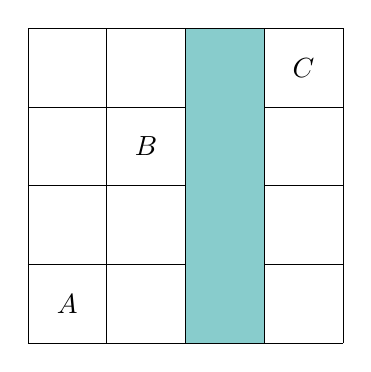
\begin{tikzpicture}
        \draw[step=1cm,black,very thin] (0,0) grid (4,4);
        \draw (0.5,0.5) node{$A$};% the y coordinates of A, B, C could be random
        \draw (1.5,2.5) node{$B$};% but I couldn't get it to work
        \draw (3.5,3.5) node{$C$};
        \filldraw[fill=color4I] (2,0) rectangle (3,4);
    \end{tikzpicture}
    \caption{Illustration for Lemma \ref{lem:RectangleBlock}: The path from $A$ to $B$ cannot be made any shorter by entering the rectangle since it could just go along the border. Meanwhile, removing the rectangle makes new paths $A$ to $C$ and $B$ to $C$.}
\end{figure}

\begin{conclusion}
And so, $\#_{1, n} = n$
\end{conclusion}

\begin{proof}
The only piece that could possibly fit is the I piece, which is removable thanks to Lemma \ref{lem:RectangleBlock}.
\end{proof}

\begin{figure}[!h]
    \centering
    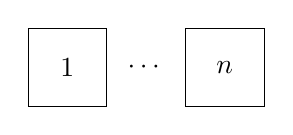
\begin{tikzpicture}
        \draw[step=1cm,black,very thin] (0,0) grid (1,1);
        \draw[step=1cm,black,very thin] (2,0) grid (3,1);
        \draw (0.5,0.5) node{1};
        \draw (1.5,0.5) node{$\cdots$};
        \draw (2.5,0.5) node{$n$};
    \end{tikzpicture}
    \caption{$\#_{1, n} = n$ (where $1 < n$).}
\end{figure}




\subsection{One pentomino}

\subsubsection{\texorpdfstring{$2 \times n$}{2 \texttimes n} grids}

\begin{corollary}[Convex border]
\label{cor:Convexborder}

Lemma \ref{lem:RectangleBlock} extends to any shape, so long as the statement "it is always shorter to go \emph{along} the border" holds. This could be a similar construction to the rectangle blockage, but it extends more generally to include, for example, some placements of pentominoes at the corner. The word "\badterm{convex}" is informal.
\end{corollary}

Consider a $2 \times n$ grid. The only pentominoes that fit are I, L, N, and Y. However, by Corollary \ref{cor:Convexborder}, L, N, and Y can be removed. So, can \minordetail{the pentomino} I be used to increase $\#^p_{2, n}$? Yes. While placing I on the corner does not help, placing the I anywhere else increases $\#^p_{2, n}$ by 1 -- the unique way to show $\#_{2, n} = n + 2$ for $n \ge 7$.

\begin{figure}[!h]
    \centering
    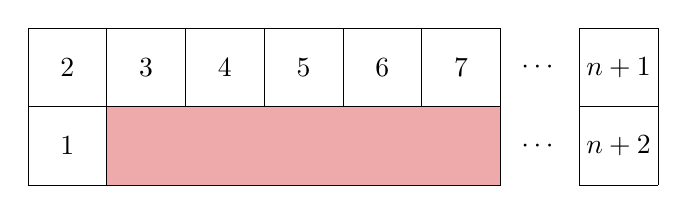
\begin{tikzpicture}
        \draw[step=1cm,black,very thin] (0,0) grid (6,2);
        \draw[step=1cm,black,very thin] (7,0) grid (8,2);
        \draw (0.5,0.5) node{1};
        \draw (0.5,1.5) node{2};
        \draw (1.5,1.5) node{3};
        \draw (2.5,1.5) node{4};
        \draw (3.5,1.5) node{5};
        \draw (4.5,1.5) node{6};
        \draw (5.5,1.5) node{7};
        \filldraw[fill=colorI] (1,0) rectangle (6,1);
        \draw (6.5,0.5) node{$\cdots$};
        \draw (6.5,1.5) node{$\cdots$};
        \draw (7.5,1.5) node{$n + 1$};
        \draw (7.5,0.5) node{$n + 2$};
    \end{tikzpicture}
    \caption{$\#_{2, n} = n + 2$ (where $7 \le n$). \cite{sheet}}
\end{figure}

\subsubsection{\texorpdfstring{$3 \times n$}{3 \texttimes n} grids}

\begin{property}[Cycle inefficiency]
\label{prop:cycineff}

If there is a cycle of empty squares in a grid, the path will not use all empty squares.
\end{property}

For $3 \times n$ grids, all pentominoes fit, but V, W, and Z can be removed by Corollary \ref{cor:Convexborder}. In the case of a $3 \times 4$ grid, we have solutions with 1 pentomino and all empty squares filled ($\#_{3, 4} = 7$, Figure \ref{fig:3x4}). Placing zero pentominoes gets a length of 6, while with two pentominoes there are only 2 leftover squares, so the only solutions have 1 pentomino and all empty squares in the path.

\begin{figure}
    \centering
    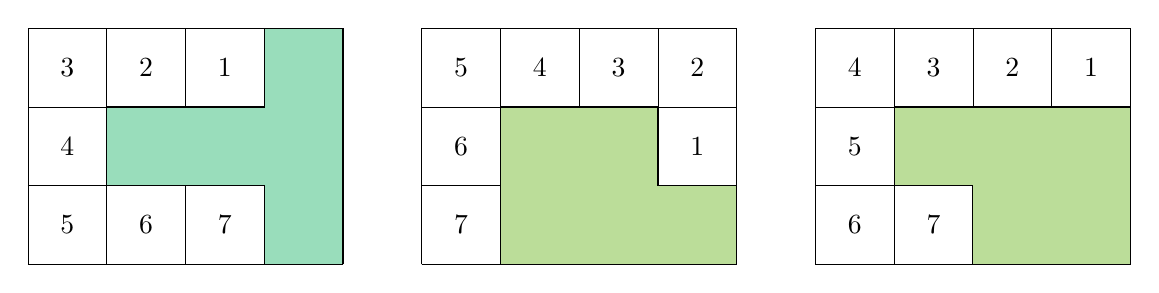
\begin{tikzpicture}
        \draw[step=1cm,black,very thin] (0,0) grid (4,3);
        \draw (2.5,2.5) node{1};
        \draw (1.5,2.5) node{2};
        \draw (0.5,2.5) node{3};
        \draw (0.5,1.5) node{4};
        \draw (0.5,0.5) node{5};
        \draw (1.5,0.5) node{6};
        \draw (2.5,0.5) node{7};
        \filldraw[fill=colorT] (3,0) -- (4,0) -- (4,3) -- (3,3) -- (3,2) -- (1,2) -- (1,1) -- (3,1) -- cycle;

        \begin{scope}[xshift=5cm]
            \draw[step=1cm,black,very thin] (0,0) grid (4,3);
            \draw (3.5,1.5) node{1};
            \draw (3.5,2.5) node{2};
            \draw (2.5,2.5) node{3};
            \draw (1.5,2.5) node{4};
            \draw (0.5,2.5) node{5};
            \draw (0.5,1.5) node{6};
            \draw (0.5,0.5) node{7};
            \filldraw[fill=colorP] (1,2) -- (1,0) -- (4,0) -- (4,1) -- (3,1) -- (3,2) -- cycle;
        \end{scope}

        \begin{scope}[xshift=10cm]
            \draw[step=1cm,black,very thin] (0,0) grid (4,3);
            \draw (3.5,2.5) node{1};
            \draw (2.5,2.5) node{2};
            \draw (1.5,2.5) node{3};
            \draw (0.5,2.5) node{4};
            \draw (0.5,1.5) node{5};
            \draw (0.5,0.5) node{6};
            \draw (1.5,0.5) node{7};
            \filldraw[fill=colorP] (1,2) -- (1,1) -- (2,1) -- (2,0) -- (4,0) -- (4,2) -- cycle;
        \end{scope}
    \end{tikzpicture}
    \caption{$\#_{3, 4} = 7$. \cite[6:04]{v2}}
    \label{fig:3x4}
\end{figure}

Pentominoes must be placed so that the grid is \emph{not} split into two. This is impossible for F and X, which span a $1 \times 3$ area with two squares padding each side of the $1 \times 3$. Pentominoes that span a $1 \times 4$ area (L, N, Y) cannot have their $1 \times 4$ in the middle, but if it is on the edge of the grid, there are two disjoint $2 \times 2$ cycles which cannot be prevented by the remaining square of the pentomino. So by \ref{prop:cycineff}, L, N, and Y are eliminated. U has 4 orientations (translations can be produced by rotation and reflection, there is 1 \minordetail{relevant} non-reflection for U, and 1 \minordetail{relevant} non-rotational symmetry for the $3 \times 4$), which all do not work for various reasons.

\begin{figure}
    \centering
    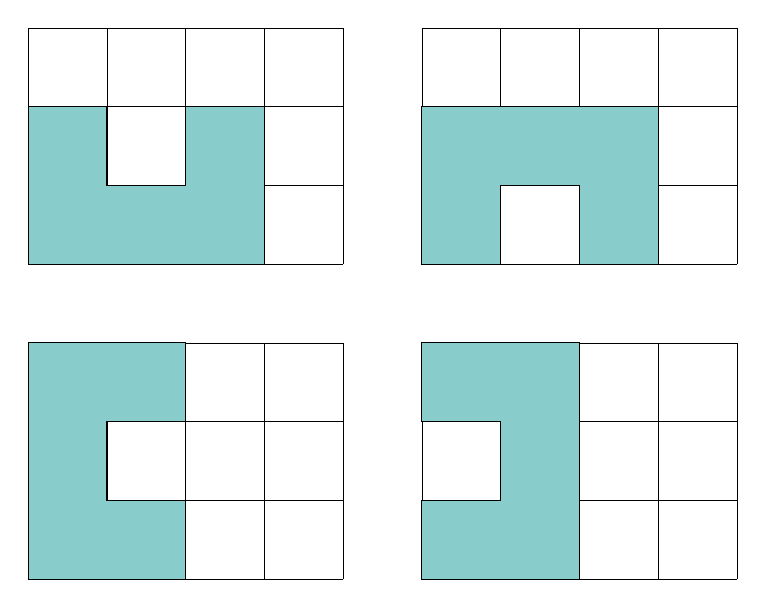
\begin{tikzpicture}
        \draw[step=1cm,black,very thin] (0,0) grid (4,3);
        \filldraw[fill=colorU] (0,0) -- (0,3) -- (2,3) -- (2,2) -- (1,2) -- (1,1) -- (2,1) -- (2,0) -- cycle;

        \begin{scope}[xshift=5cm]
            \draw[step=1cm,black,very thin] (0,0) grid (4,3);
            \filldraw[fill=colorU] (0,0) -- (0,1) -- (1,1) -- (1,2) -- (0,2) -- (0,3) -- (2,3) -- (2,0) -- cycle;
        \end{scope}

        \begin{scope}[yshift=4cm]
            \draw[step=1cm,black,very thin] (0,0) grid (4,3);
            \filldraw[fill=colorU] (0,0) -- (3,0) -- (3,2) -- (2,2) -- (2,1) -- (1,1) -- (1,2) -- (0,2) -- cycle;
        \end{scope}

        \begin{scope}[shift={(5cm,4cm)}]
            \draw[step=1cm,black,very thin] (0,0) grid (4,3);
            \filldraw[fill=colorU] (0,0) -- (1,0) -- (1,1) -- (2,1) -- (2,0) -- (3,0) -- (3,2) -- (0,2) -- cycle;
        \end{scope}
    \end{tikzpicture}
    \caption{Orientations of U in a $3 \times 4$ (footnote: \protect\footnotemark)}
\end{figure}

\footnotetext{film2860 on discord used gpt-4o to try to remove pixel artifacts. It generated equivalent code, which did not fix the problem, but did illustrate the usage of scopes which was helpful as a beginner. So congrats on contributing!}

We are left with the pentominoes P and T. If P does not touch the corner, after placing the $2 \times 2$, the 5th square must divide the grid in two. There are four ways to touch the corner, and two work. For T, there is only one orientation that does not split the grid in two. So the three solutions given by \cite[6:04]{v2} are the only ones.

% Informally, we define a pentomino's \newterm{contribution} to be how much it lengthens a particular path.

% \subsection{How to add Tables}

% Use the table and tabular environments for basic tables --- see Table~\ref{tab:widgets}, for example. For more information, please see this help article on \href{https://www.overleaf.com/learn/latex/tables}{tables}.

% \begin{table}
% \centering
% \begin{tabular}{l|r}
% Item & Quantity \\\hline
% Widgets & 42 \\
% Gadgets & 13
% \end{tabular}
% \caption{\label{tab:widgets}An example table.}
% \end{table}

% \subsection{How to add Comments and Track Changes}

% Comments can be added to your project by highlighting some text and clicking ``Add comment'' in the top right of the editor pane. To view existing comments, click on the Review menu in the toolbar above. To reply to a comment, click on the Reply button in the lower right corner of the comment. You can close the Review pane by clicking its name on the toolbar when you're done reviewing for the time being.

% Track changes are available on all our \href{https://www.overleaf.com/user/subscription/plans}{premium plans}, and can be toggled on or off using the option at the top of the Review pane. Track changes allow you to keep track of every change made to the document, along with the person making the change.

% \subsection{How to add Lists}

% You can make lists with automatic numbering \dots

% \begin{enumerate}
% \item Like this,
% \item and like this.
% \end{enumerate}
% \dots or bullet points \dots
% \begin{itemize}
% \item Like this,
% \item and like this.
% \end{itemize}

% \subsection{How to write Mathematics}

% \LaTeX{} is great at typesetting mathematics. Let $X_1, X_2, \ldots, X_n$ be a sequence of independent and identically distributed random variables with $\text{E}[X_i] = \mu$ and $\text{Var}[X_i] = \sigma^2 < \infty$, and let
% \[S_n = \frac{X_1 + X_2 + \cdots + X_n}{n}
%       = \frac{1}{n}\sum_{i}^{n} X_i\]
% denote their mean. Then as $n$ approaches infinity, the random variables $\sqrt{n}(S_n - \mu)$ converge in distribution to a normal $\mathcal{N}(0, \sigma^2)$.


% \subsection{How to change the margins and paper size}

% Usually the template you're using will have the page margins and paper size set correctly for that use-case. For example, if you're using a journal article template provided by the journal publisher, that template will be formatted according to their requirements. In these cases, it's best not to alter the margins directly.

% If however you're using a more general template, such as this one, and would like to alter the margins, a common way to do so is via the geometry package. You can find the geometry package loaded in the preamble at the top of this example file, and if you'd like to learn more about how to adjust the settings, please visit this help article on \href{https://www.overleaf.com/learn/latex/page_size_and_margins}{page size and margins}.

% \subsection{How to change the document language and spell check settings}

% Overleaf supports many different languages, including multiple different languages within one document.

% To configure the document language, simply edit the option provided to the babel package in the preamble at the top of this example project. To learn more about the different options, please visit this help article on \href{https://www.overleaf.com/learn/latex/International_language_support}{international language support}.

% To change the spell check language, simply open the Overleaf menu at the top left of the editor window, scroll down to the spell check setting, and adjust accordingly.

% \subsection{Good luck!}

% We hope you find Overleaf useful, and do take a look at our \href{https://www.overleaf.com/learn}{help library} for more tutorials and user guides! Please also let us know if you have any feedback using the Contact Us link at the bottom of the Overleaf menu --- or use the contact form at \url{https://www.overleaf.com/contact}.

\printbibliography

\end{document}